\section{Formal Analysis}
\subsection{Alloy code}


\begin{lstlisting}[language=alloy]
-- SIGNATURES

-- Basic types
sig Location {}

-- Enumerations for path status
abstract sig PathStatus {}
one sig Optimal extends PathStatus {}
one sig Medium extends PathStatus {}
one sig RequiresMaintenance extends PathStatus {}

-- Enumerations for anomaly types
abstract sig AnomalyType {}
one sig Pothole extends AnomalyType {}
one sig RoughSurface extends AnomalyType {}
one sig Obstacle extends AnomalyType {}

-- Enumerations for verification status
abstract sig VerificationStatus {}
one sig Pending extends VerificationStatus {}
one sig Confirmed extends VerificationStatus {}
one sig Rejected extends VerificationStatus {}

-- Enumerations for visibility
abstract sig Visibility {}
one sig PrivateVis extends Visibility {}
one sig PublicVis extends Visibility {}

-- Boolean type
abstract sig Bool {}
one sig True extends Bool {}
one sig False extends Bool {}

-- Users
sig RegisteredUser {
    trips : set Trip,
    manualReports : set PathReport
}

-- Physical path segment in the world
sig PathSegment {
    location : one Location,
    publishedReports : set PathReport
}

-- Trip recorded by a user
sig Trip {
    owner : one RegisteredUser,
    path : set PathSegment,
    detectedAnomalies : set SensorAnomaly,
    visibility : one Visibility
}

-- Automated sensor data
sig SensorAnomaly {
    tripContext : one Trip,
    anomalyType : one AnomalyType,
    anomalyLocation : one Location,
    verification : one VerificationStatus,
    resultingReport : lone PathReport
}

-- Validated path information
sig PathReport {
    reporter : one RegisteredUser,
    segment : one PathSegment,
    statusReported : one PathStatus,
    isAutomated : one Bool,
    visibility : one Visibility
}

-- Route visualization
sig Route {
    segments : some PathSegment
}


-- FACTS

-- F1: Trip Ownership
fact TripOwnership {
    all t: Trip | t in t.owner.trips
    all u: RegisteredUser, t: Trip | t in u.trips iff t.owner = u
}

-- F2: Anomaly Context
fact AnomalyBelongsToTrip {
    all a: SensorAnomaly | a in a.tripContext.detectedAnomalies
}

-- F3: Report Authorship
fact ReportAuthorship {
    all r: PathReport | {
        (r.isAutomated = True implies 
            (one a: SensorAnomaly | 
                a.resultingReport = r and 
                a.tripContext.owner = r.reporter))
        and
        (r.isAutomated = False implies r in r.reporter.manualReports)
    }
}

-- F4: Verification Logic
fact VerificationLogic {
    all a: SensorAnomaly | {
        (a.verification = Confirmed iff one r: PathReport | r = a.resultingReport)
        and
        ((a.verification = Pending or a.verification = Rejected) 
            implies no a.resultingReport)
        and
        (some a.resultingReport implies 
            a.resultingReport.reporter = a.tripContext.owner)
    }
}

-- F5: Location Consistency
fact LocationConsistency {
    all a: SensorAnomaly, r: PathReport |
        a.resultingReport = r implies r.segment.location = a.anomalyLocation
}

-- F6: Trip Geography
fact AnomalyOnPath {
    all a: SensorAnomaly |
        some s: PathSegment | 
            s in a.tripContext.path and 
            s.location = a.anomalyLocation
}

-- F7: Privacy by Default
fact PrivacyByDefault {
    all t: Trip | (t.visibility = PrivateVis or t.visibility = PublicVis)
}

-- F8: Privacy Inheritance for Automated Reports
fact PrivacyInheritance {
    all a: SensorAnomaly, r: PathReport |
        (a.resultingReport = r and a.tripContext.visibility = PrivateVis) 
        implies r.visibility = PrivateVis
}

-- F9: Published Reports Visibility
fact PublishedReportsArePublic {
    all s: PathSegment, r: PathReport |
        r in s.publishedReports implies r.visibility = PublicVis
}

-- F10: Manual Report Ownership
fact ManualReportOwnership {
    all r: PathReport |
        r.isAutomated = False implies r in r.reporter.manualReports
}

-- F11: No Duplicate Reports
fact NoDuplicateReports {
    all u: RegisteredUser, s: PathSegment |
        lone r: PathReport | 
            r.reporter = u and 
            r.segment = s and 
            r in s.publishedReports
}

-- F12: Routes Use Segments with Data
fact RoutesHavePublishedData {
    all r: Route, s: r.segments | 
        #(s.publishedReports) > 0
}

-- F13: All locations connected
fact AllLocationsConnected {
    all loc: Location | one s: PathSegment | loc = s.location
}

-- F14: All reports connected
fact AllReportsConnected {
    all r: PathReport | {
        (r.isAutomated = True implies one a: SensorAnomaly | a.resultingReport = r)
        or
        (r.isAutomated = False implies one u: RegisteredUser | r in u.manualReports)
    }
}

-- F15: All anomalies connected
fact AllAnomaliesConnected {
    all a: SensorAnomaly | one t: Trip | a in t.detectedAnomalies
}


-- ASSERTIONS - VERIFY CORE REQUIREMENTS

-- A1: No rejected anomalies create reports
assert NoRejectedReports {
    all a: SensorAnomaly | 
        a.verification = Rejected implies no a.resultingReport
}

-- A2: All automated reports come from confirmed anomalies
assert AutomatedReportsAreVerified {
    all r: PathReport | 
        r.isAutomated = True implies
        (one a: SensorAnomaly | 
            a.resultingReport = r and 
            a.verification = Confirmed)
}

-- A3: Privacy guarantee
assert PrivacyGuarantee {
    all t: Trip | 
        t.visibility = PrivateVis implies
        (all a: t.detectedAnomalies |
            (some a.resultingReport) implies 
            a.resultingReport.visibility = PrivateVis)
}

-- A4: Published reports are only public
assert NoPrivateInPublishedInventory {
    all s: PathSegment, r: s.publishedReports | 
        r.visibility = PublicVis
}

-- A5: Every report has an author
assert AllReportsHaveAuthor {
    all r: PathReport | one u: RegisteredUser | r.reporter = u
}

-- A6: Anomalies are only on traveled paths
assert AnomaliesOnTraveledPaths {
    all a: SensorAnomaly |
        some s: a.tripContext.path | s.location = a.anomalyLocation
}

-- A7: No orphan trips
assert NoOrphanTrips {
    all t: Trip | one u: RegisteredUser | t.owner = u
}

-- A8: Pending anomalies await user action
assert PendingAnomaliesNoReports {
    all a: SensorAnomaly |
        a.verification = Pending implies no a.resultingReport
}

-- Checks

check NoRejectedReports for 5
check AutomatedReportsAreVerified for 5
check PrivacyGuarantee for 5
check NoPrivateInPublishedInventory for 5
check AllReportsHaveAuthor for 5
check AnomaliesOnTraveledPaths for 5
check NoOrphanTrips for 5
check PendingAnomaliesNoReports for 5


-- PREDICATES

-- S1: Manual insertion of path information
pred Scenario_ManualPathReporting {
    some u: RegisteredUser, s: PathSegment, r: PathReport | {
        r in u.manualReports
        r.reporter = u
        r.segment = s
        r.isAutomated = False
        r.statusReported = RequiresMaintenance
        r.visibility = PublicVis
        r in s.publishedReports
    }
}

-- S2: Automated detection with confirmation
pred Scenario_AutomatedDetectionConfirmed {
    some u: RegisteredUser, t: Trip, a: SensorAnomaly, s: PathSegment, r: PathReport | {
        t.owner = u
        s in t.path
        a in t.detectedAnomalies
        a.tripContext = t
        a.anomalyLocation = s.location
        a.anomalyType = Pothole
        a.verification = Confirmed
        a.resultingReport = r
        r.reporter = u
        r.segment = s
        r.isAutomated = True
        r.visibility = PublicVis
        r in s.publishedReports
    }
}

-- S3: False positive rejection (CORE for Group 2)
pred Scenario_FalsePositiveRejected {
    some u: RegisteredUser, t: Trip, a: SensorAnomaly | {
        t.owner = u
        a in t.detectedAnomalies
        a.tripContext = t
        a.anomalyType = Pothole
        a.verification = Rejected
        no a.resultingReport
        no r: PathReport | 
            r.isAutomated = True and 
            r.reporter = u and
            r.segment.location = a.anomalyLocation
    }
}

-- S4: Private trip with pending anomalies
pred Scenario_PrivateTripWithPendingAnomalies {
    some u: RegisteredUser, t: Trip, a: SensorAnomaly | {
        t.owner = u
        t.visibility = PrivateVis
        a in t.detectedAnomalies
        a.tripContext = t
        a.verification = Pending
        no a.resultingReport
        no r: PathReport | r.reporter = u and r in PathSegment.publishedReports
    }
}



-- S5: User publishes previously private data
pred Scenario_PublishPrivateData {
    some u: RegisteredUser, t: Trip, a: SensorAnomaly, r: PathReport, s: PathSegment | {
        t.owner = u
        t.visibility = PrivateVis
        a in t.detectedAnomalies
        a.verification = Confirmed
        a.resultingReport = r
        r.visibility = PublicVis
        r.segment = s
        r in s.publishedReports
        t.visibility = PrivateVis
    }
}

-- S6: Route visualization
pred Scenario_RouteVisualization {
    some route: Route | {
        #(route.segments) >= 2
        all s: route.segments | 
            #(s.publishedReports) > 0
        #(route.segments.publishedReports.reporter) >= 1
    }
}

-- S7: Multiple users contribute data
pred Scenario_MultipleContributors {
    some s: PathSegment, r1, r2: PathReport, u1, u2: RegisteredUser | {
        u1 != u2
        r1.segment = s and r2.segment = s
        r1.reporter = u1 and r2.reporter = u2
        r1 in s.publishedReports
        r2 in s.publishedReports
        r1.statusReported != r2.statusReported
    }
}


-- WORLDS

--  Used to not show orphans PathSegments in worlds
pred CleanWorld {
    all s: PathSegment | (some t: Trip | s in t.path) or (some r: PathReport | r.segment = s)
}

-- World showing the confirmation workflow
pred World_ConfirmationWorkflow {
    some u: RegisteredUser, t: Trip | {
        t.owner = u
        #(t.detectedAnomalies) = 3
        one a1: t.detectedAnomalies | a1.verification = Confirmed
        one a2: t.detectedAnomalies | a2.verification = Rejected  
        one a3: t.detectedAnomalies | a3.verification = Pending
        #{a: t.detectedAnomalies | some a.resultingReport} = 1
    }
}

-- World 1: Simple registration (initial state)
pred World1 {
    #RegisteredUser = 2
    #Trip = 0
    #PathReport = 0
    #SensorAnomaly = 0
}

-- World 2: Manual reporting only
pred World2 {
    #RegisteredUser = 2
    #Trip = 2
    #PathSegment = 3
    #PathReport > 1
    #SensorAnomaly = 0
    // All reports are manual
    all r: PathReport | r.isAutomated = False
}

-- World 3: Automated detection with confirmation
pred World3 {
    #RegisteredUser = 1
    #Trip = 1
    #SensorAnomaly = 2
    #PathReport > 0
    // At least one anomaly confirmed
    some a: SensorAnomaly | a.verification = Confirmed
}

-- World 4: Mixed manual and automated reports
pred World4_MixedReports {
    some u: RegisteredUser, t: Trip, s1, s2: PathSegment, r1, r2: PathReport | {
        t.owner = u
        s1 != s2
        
        // Manual report
        r1 in u.manualReports
        r1.isAutomated = False
        r1.segment = s1
        r1.visibility = PublicVis
        r1 in s1.publishedReports
        
        // Automated report from confirmed anomaly
        some a: t.detectedAnomalies | {
            a.verification = Confirmed
            a.resultingReport = r2
            r2.segment = s2
            r2.isAutomated = True
            r2.visibility = PublicVis
            r2 in s2.publishedReports
        }
    }
}

-- World 5: Privacy demonstration
pred World5_PrivateVsPublic {
    some u: RegisteredUser, t1, t2: Trip | {
        t1.owner = u
        t2.owner = u
        t1 != t2
        
        // Private trip with pending anomalies
        t1.visibility = PrivateVis
        some a1: t1.detectedAnomalies | a1.verification = Pending
        
        // Public trip with confirmed and published data
        t2.visibility = PublicVis
        some a2: t2.detectedAnomalies | {
            a2.verification = Confirmed
            some a2.resultingReport
            a2.resultingReport.visibility = PublicVis
        }
    }
}

-- Execution Commands
run World1_Clean { World1 and CleanWorld } for 5
run World2_Clean { World2 and CleanWorld } for 5
run World3_Clean { World3 and CleanWorld } for 5
run World4_Clean { World4_MixedReports and CleanWorld } for 5
run World5_Clean { World5_PrivateVsPublic and CleanWorld } for 5
run Workflow_Clean { World_ConfirmationWorkflow and CleanWorld } for 5
\end{lstlisting}

\subsubsection{Worlds}

The following instances (Worlds) have been generated to visually validate the consistency of the model against specific functional scenarios. Each world represents a snapshot of the system state satisfying a distinct set of constraints.

\paragraph{World 1: Initial System State} This instance represents the baseline state of the BBP system. It depicts the existence of registered users prior to the creation of any trips, anomalies, or reports. This world confirms that the static structural constraints of the domain model are consistent even in the absence of dynamic activity.

\begin{figure}[H] \begin{center} 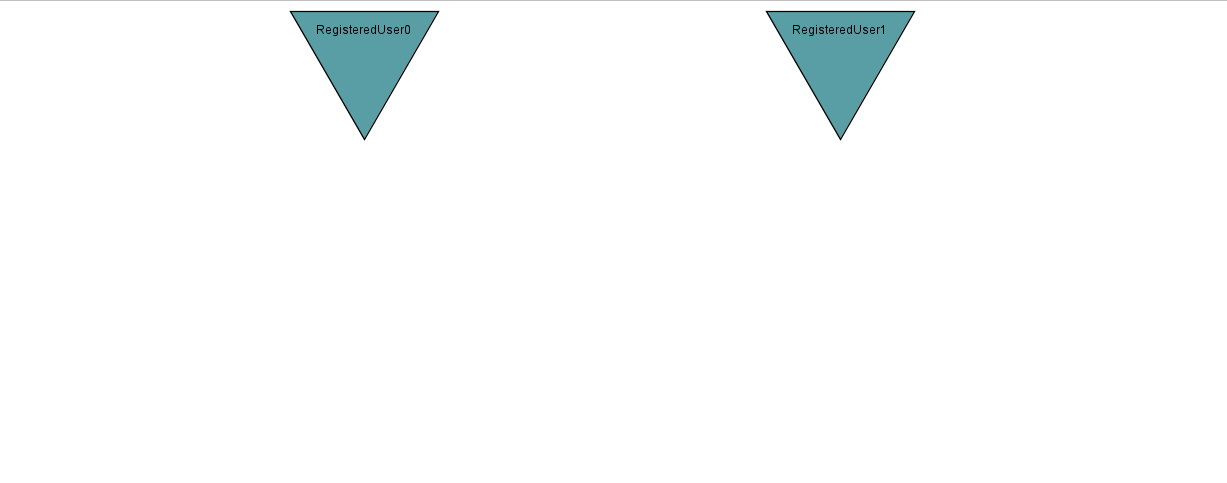
\includegraphics[width=\textwidth]{RASD/img/section4/world1.png} \caption{World 1: Initial State with registered users but no activity.} \end{center} \end{figure}

\newpage

\paragraph{World 2: Manual Reporting Workflow} This scenario illustrates the system's behavior when relying exclusively on user inputs. It depicts a state containing multiple trips and path reports, where all reports are explicitly marked as manual (isAutomated = False). This world validates that the system can successfully manage crowdsourced data without requiring the intervention of the automated sensor subsystem.

\begin{figure}[H] \begin{center} 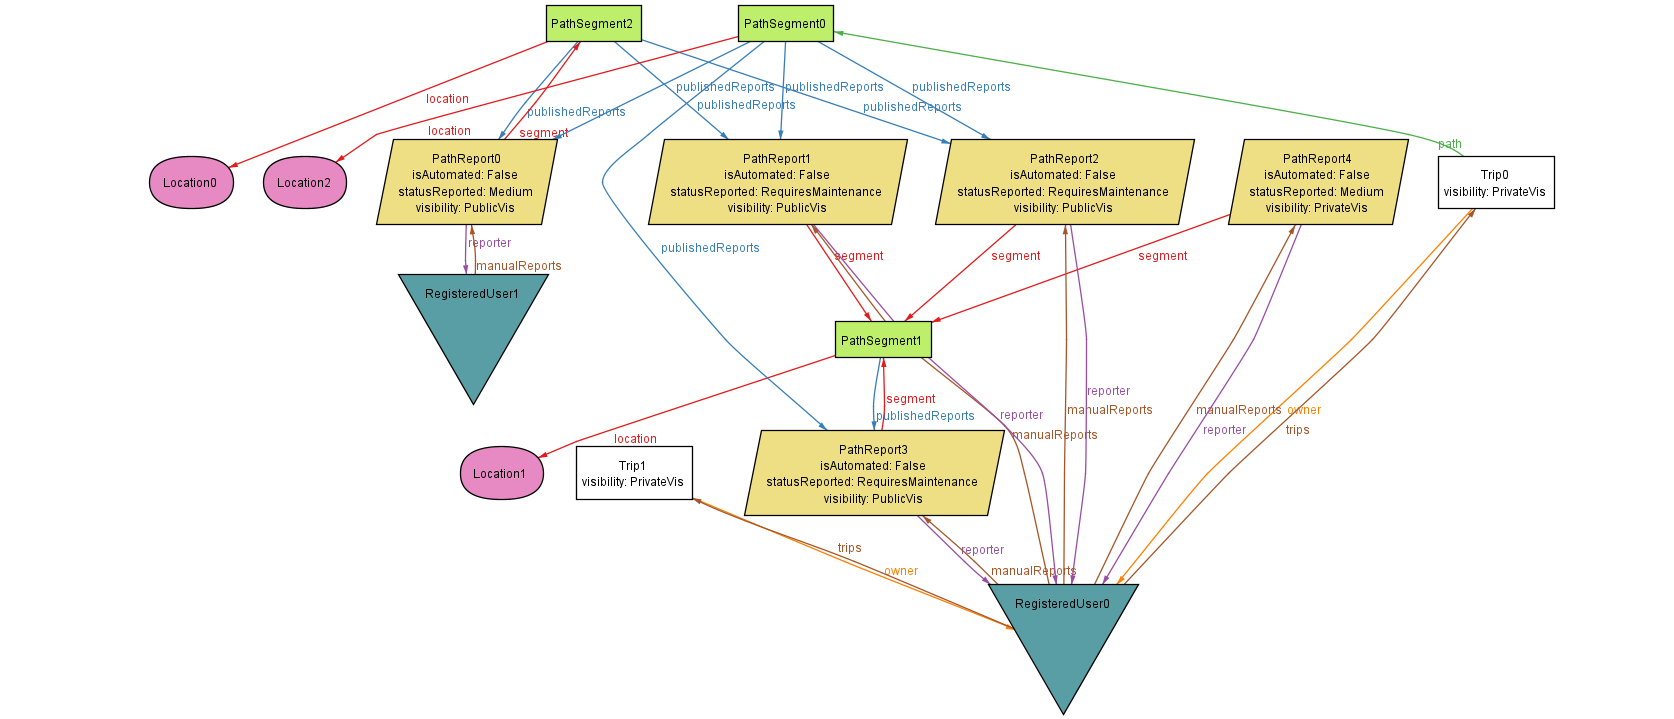
\includegraphics[width=\textwidth]{RASD/img/section4/world2.png} \caption{World 2: Scenario focusing on Manual Reporting only.} \end{center} \end{figure}

\newpage

\paragraph{World 3: Automated Detection and Verification} This instance focuses on the lifecycle of automatically detected data. It shows the generation of SensorAnomaly entities linked to a trip and verifies the transition logic where a user confirms an anomaly, resulting in the creation of a valid PathReport. This world is essential to verify that the automated collection and user verification loop functions correctly.

\begin{figure}[H] \begin{center} 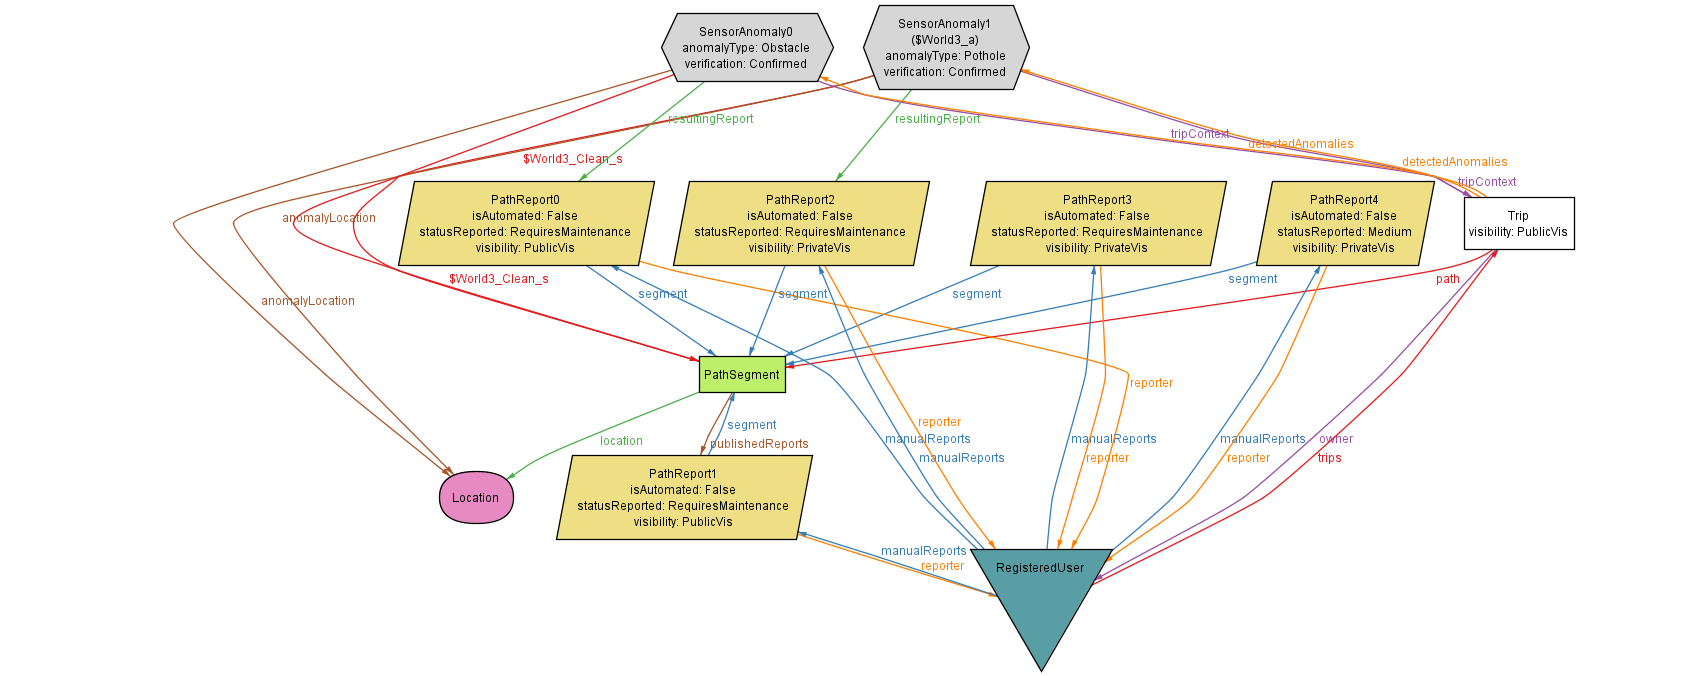
\includegraphics[width=\textwidth]{RASD/img/section4/world3.png} \caption{World 3: Scenario showing Automated Detection and Verification.} \end{center} \end{figure}

\newpage

\paragraph{World 4: Aggregation of Heterogeneous Data} This world demonstrates the system's capability to integrate different data sources simultaneously. It presents a complex state where manual reports coexist with automated reports derived from confirmed sensor anomalies. This validation ensures that the PathReport entity correctly abstracts the data origin (manual vs. automated) while maintaining consistency in the public inventory.

\begin{figure}[H] \begin{center} 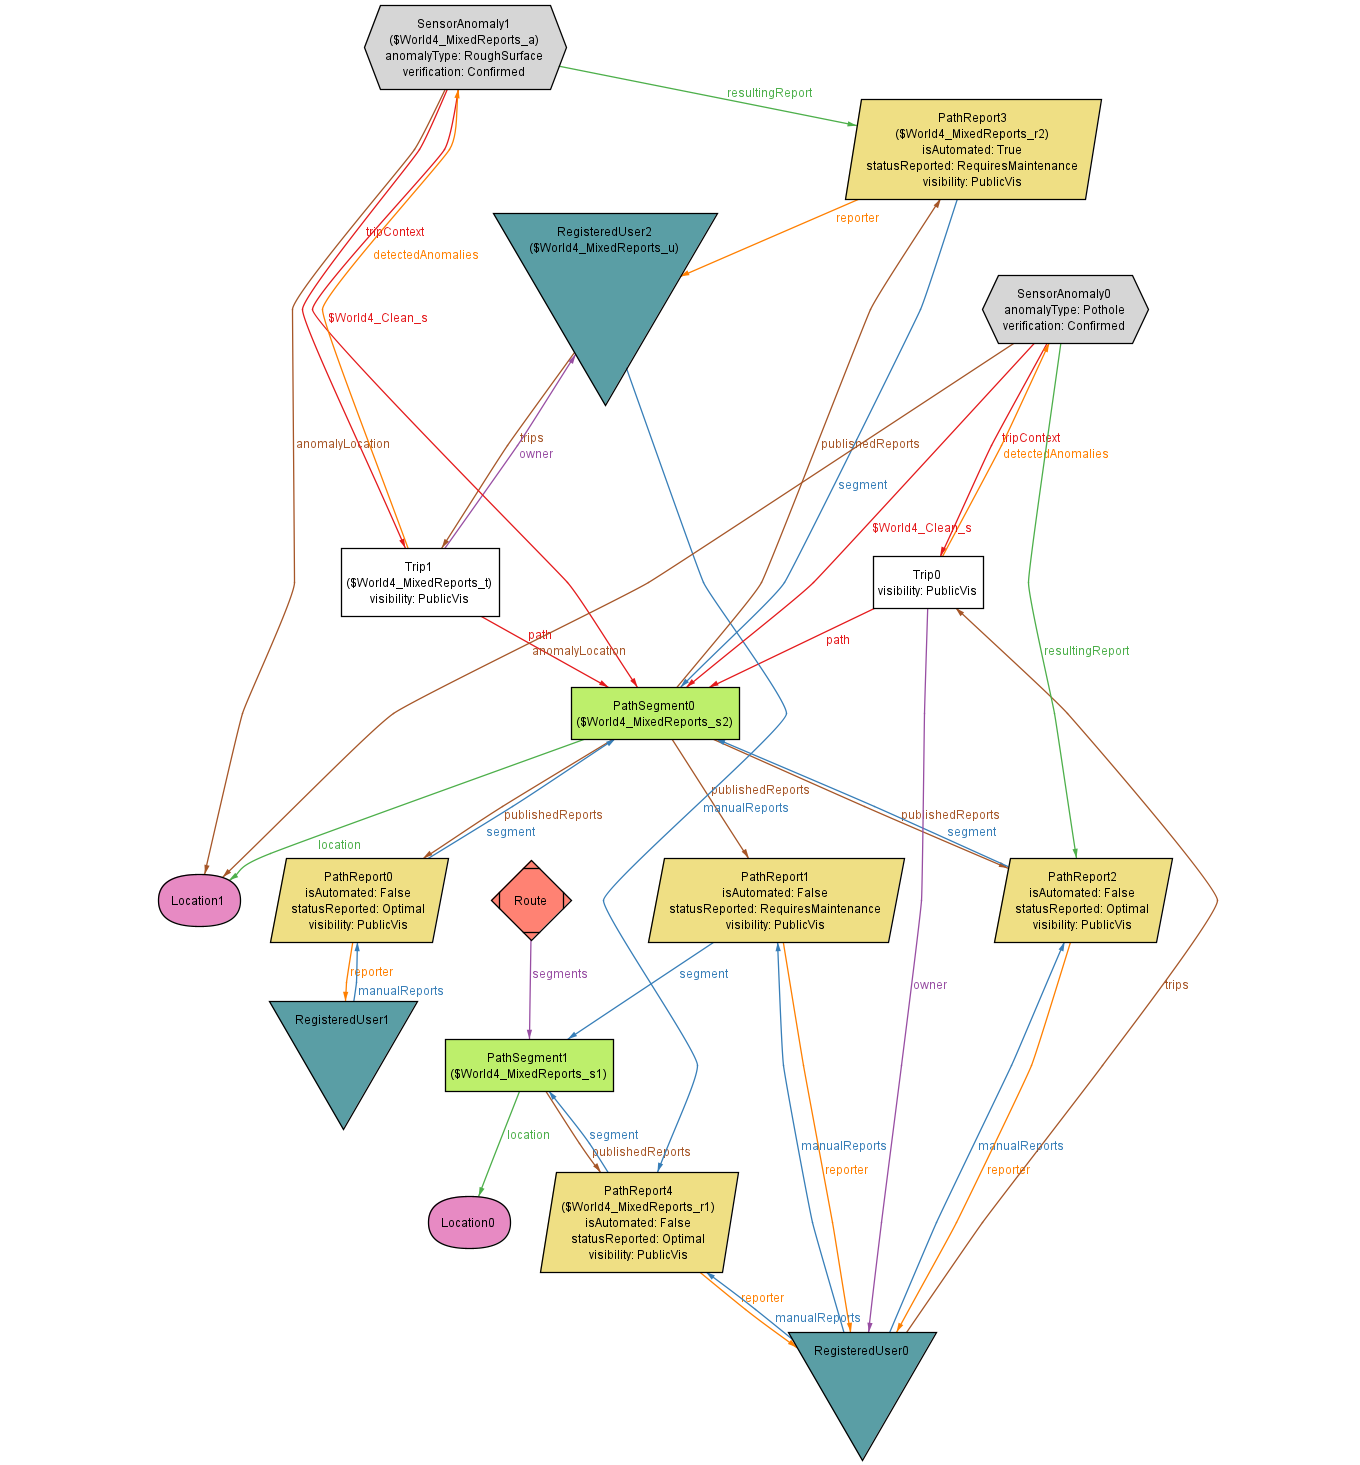
\includegraphics[width=\textwidth]{RASD/img/section4/world4.png} \caption{World 4: Coexistence of Manual and Automated reports.} \end{center} \end{figure}

\newpage

\paragraph{World 5: Privacy Constraints} This scenario validates the "Privacy by Default" requirement and the explicit publication mechanism. It contrasts two distinct trips owned by the same user: a \textit{Private} trip, where detected anomalies remain pending and isolated, and a \textit{Public} trip, where confirmed data is visible to the community. This world proves that the model correctly enforces visibility boundaries, preventing the accidental leakage of private user data.

\begin{figure}[H] \begin{center} 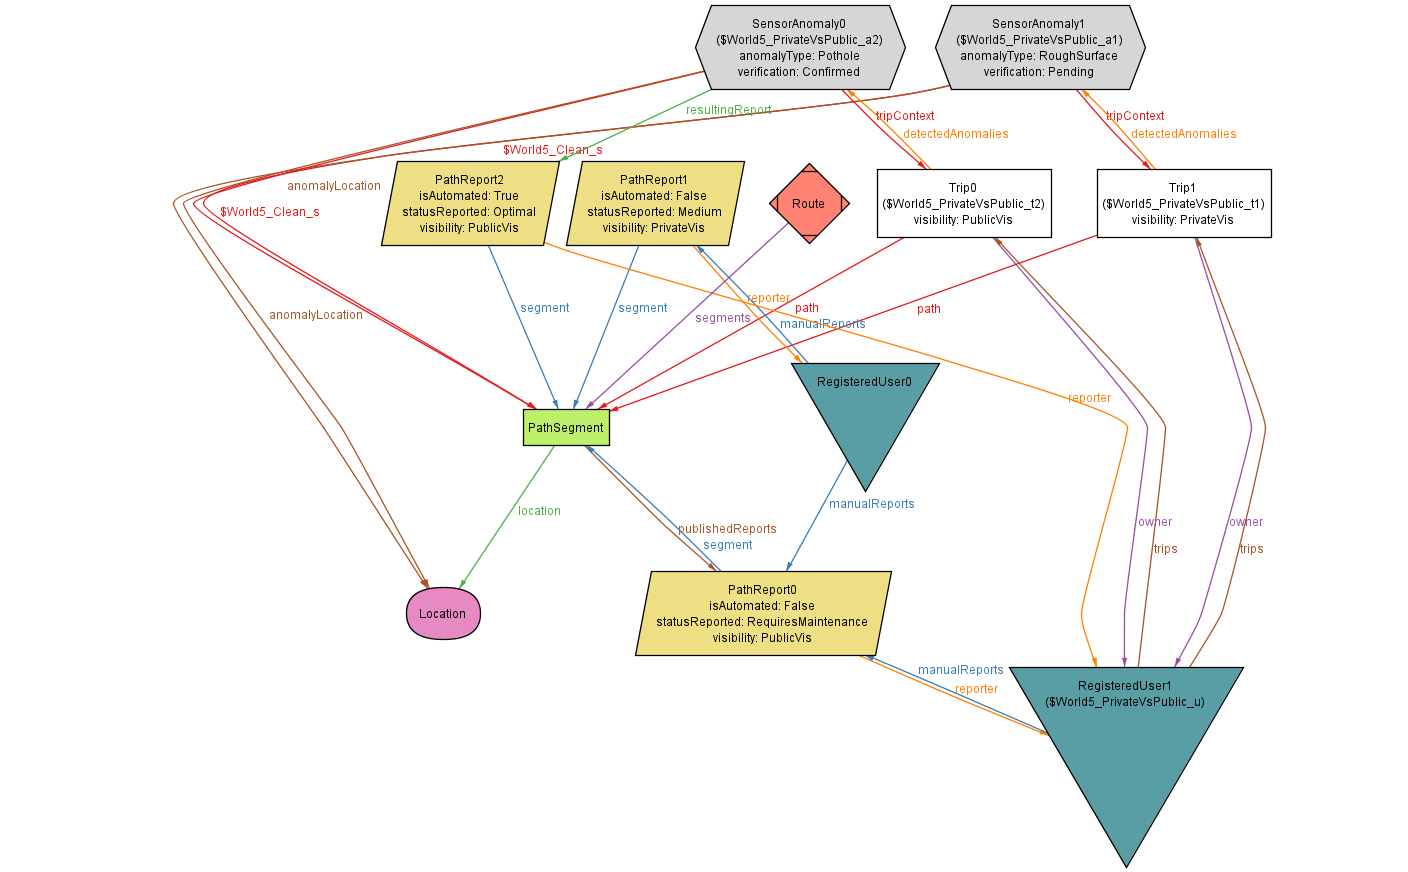
\includegraphics[width=\textwidth]{RASD/img/section4/world5.png} \caption{World 5: Privacy mechanisms and data publication.} \end{center} \end{figure}
\newpage

\paragraph{Anomaly Verification Workflow} This specific instance validates the lifecycle of sensor data, showcasing the three possible states of an anomaly within a single trip. It depicts a scenario where multiple anomalies coexist: one confirmed (generating a report), one rejected (discarded), and one pending (awaiting action). This visualizes the correctness of the state machine logic formalized in Fact F4, ensuring that only verified data impacts the public inventory.

\begin{figure}[H] \begin{center} 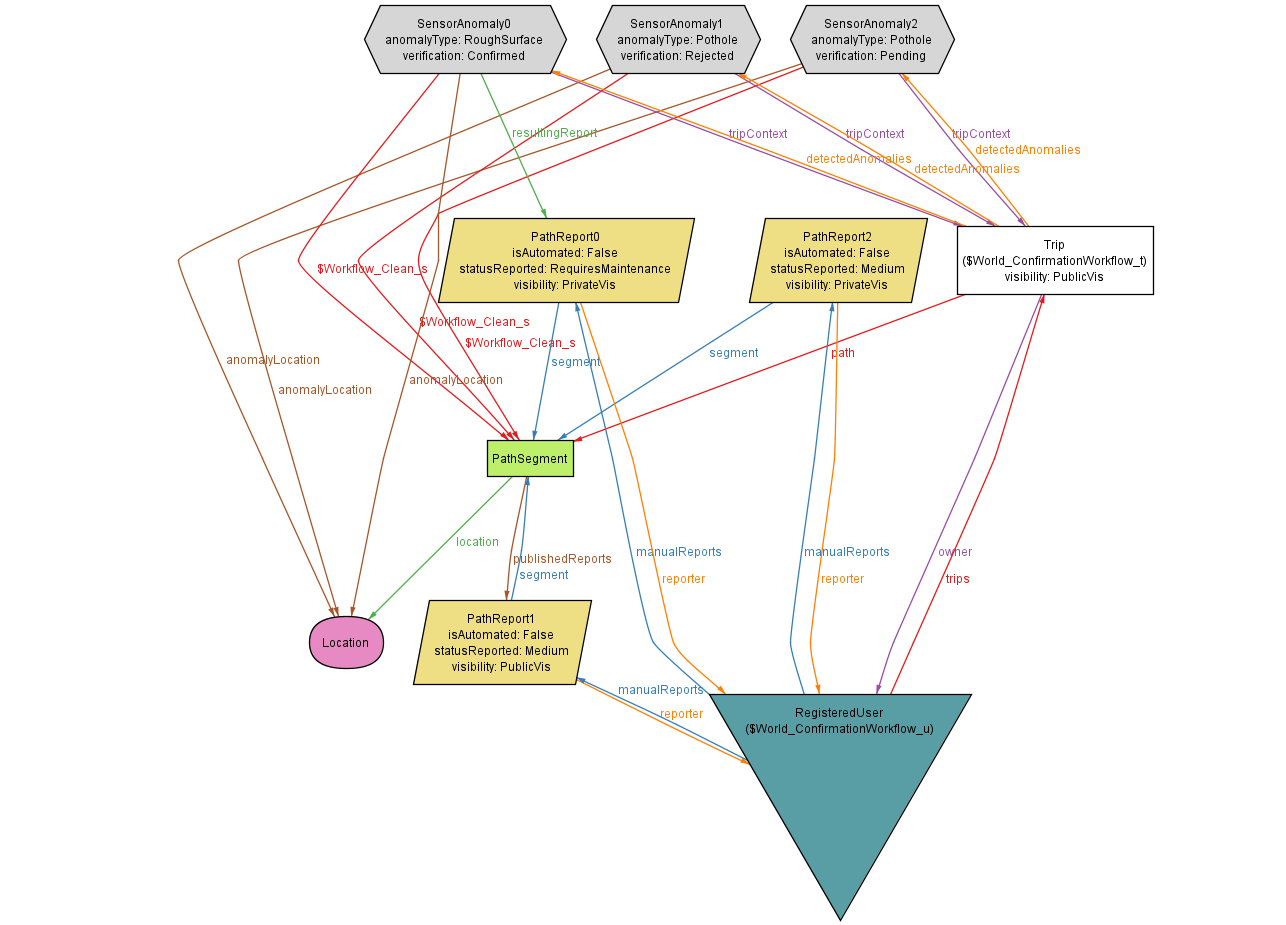
\includegraphics[width=\textwidth]{RASD/img/section4/workflow.png} \caption{Verification Workflow: Handling Pending, Confirmed, and Rejected anomalies.} \end{center} \end{figure}